\documentclass[conference]{IEEEtran}
\IEEEoverridecommandlockouts
\usepackage{cite}
\usepackage{amsmath,amssymb,amsfonts}
\usepackage{graphicx}
\usepackage{textcomp}
\usepackage{xcolor}
\usepackage{booktabs}
\usepackage{hyperref}

% AUTO-GENERATED by src/evaluation/generate_latex_tables.py. Do not edit by hand.
\newcommand{\MaxClusterDistKm}{34.9}
\newcommand{\MeanNOx}{528.6}
\newcommand{\MeanWindSpeed}{3.76}
\newcommand{\MedianNOx}{443.0}
\newcommand{\MinDetectableEffectKgH}{19.6}
\newcommand{\MinDetectableEffectPct}{9.1}
\newcommand{\NAdvTestWindows}{14,421}
\newcommand{\NCalmTestWindows}{3,877}
\newcommand{\NClusters}{16}
\newcommand{\NFacAirCrossBest}{1}
\newcommand{\NFacGBBest}{3}
\newcommand{\NFacGlobalBest}{2}
\newcommand{\NFacLoadRegBest}{5}
\newcommand{\NFacOh}{4}
\newcommand{\NFacPa}{2}
\newcommand{\NFacTx}{13}
\newcommand{\NFacilities}{19}
\newcommand{\NFacilityHours}{83,296}
\newcommand{\NFolds}{5}
\newcommand{\NMidwestPlants}{6}
\newcommand{\NMidwestTestWindows}{5,617}
\newcommand{\NMissingNOxHours}{0}
\newcommand{\NNonOperatingHours}{10,998}
\newcommand{\NOperatingHours}{72,298}
\newcommand{\NSeeds}{5}
\newcommand{\NTxPlants}{13}
\newcommand{\NTxTestWindows}{12,681}
\newcommand{\NWindows}{66,730}
\newcommand{\RegimeAirCrossAdvGainMAE}{18.4}
\newcommand{\RegimeAirCrossAdvMAE}{163.2}
\newcommand{\RegimeAirCrossCalmMAE}{181.6}
\newcommand{\RegimeAirCrossMidwestGainMAE}{100.0}
\newcommand{\RegimeAirCrossMidwestMAE}{202.9}
\newcommand{\RegimeAirCrossMidwestVsLoadRegPct}{33.0}
\newcommand{\RegimeAirCrossTxMAE}{151.2}
\newcommand{\RegimeFacMeanAdvMAE}{252.1}
\newcommand{\RegimeFacMeanCalmMAE}{285.6}
\newcommand{\RegimeFacMeanMidwestMAE}{301.3}
\newcommand{\RegimeFacMeanTxMAE}{240.6}
\newcommand{\RegimeGBAdvMAE}{158.6}
\newcommand{\RegimeGBCalmMAE}{165.9}
\newcommand{\RegimeGBMidwestGainMAE}{96.0}
\newcommand{\RegimeGBMidwestMAE}{206.9}
\newcommand{\RegimeGBMidwestVsLoadRegPct}{31.7}
\newcommand{\RegimeGBTxMAE}{139.4}
\newcommand{\RegimeLoadRegAdvGainMAE}{30.5}
\newcommand{\RegimeLoadRegAdvMAE}{202.7}
\newcommand{\RegimeLoadRegCalmMAE}{233.2}
\newcommand{\RegimeLoadRegMidwestMAE}{302.9}
\newcommand{\RegimeLoadRegTxMAE}{167.6}
\newcommand{\RegimeMWDiffAirCrossGBhi}{24.1}
\newcommand{\RegimeMWDiffAirCrossGBlo}{-30.5}
\newcommand{\RegimeTXDiffAirCrossGBhi}{23.5}
\newcommand{\RegimeTXDiffAirCrossGBlo}{2.3}
\newcommand{\RunID}{20261020\_141142}
\newcommand{\SelMinHours}{300}
\newcommand{\SelMinNOx}{200}
\newcommand{\SpatAirCrossBias}{-36.6}
\newcommand{\SpatAirCrossCIhi}{275.2}
\newcommand{\SpatAirCrossCIlo}{167.8}
\newcommand{\SpatAirCrossMAE}{217.5}
\newcommand{\SpatAirCrossMAEsd}{5.8}
\newcommand{\SpatAirCrossNoXBias}{-14.1}
\newcommand{\SpatAirCrossNoXCIhi}{271.0}
\newcommand{\SpatAirCrossNoXCIlo}{166.6}
\newcommand{\SpatAirCrossNoXMAE}{214.6}
\newcommand{\SpatAirCrossNoXMAEsd}{3.0}
\newcommand{\SpatAirCrossNoXR}{0.347}
\newcommand{\SpatAirCrossNoXRMSE}{308.0}
\newcommand{\SpatAirCrossNoXdCIhi}{+14.2}
\newcommand{\SpatAirCrossNoXdCIlo}{-17.3}
\newcommand{\SpatAirCrossNoXlogMAE}{0.431}
\newcommand{\SpatAirCrossR}{0.318}
\newcommand{\SpatAirCrossRMSE}{314.8}
\newcommand{\SpatAirCrossVsGlobalPct}{28.6}
\newcommand{\SpatAirCrossVsLoadRegPct}{-0.5}
\newcommand{\SpatAirCrossWBias}{-50.3}
\newcommand{\SpatAirCrossWCIhi}{361.7}
\newcommand{\SpatAirCrossWCIlo}{251.6}
\newcommand{\SpatAirCrossWMAE}{299.7}
\newcommand{\SpatAirCrossWMAEsd}{3.6}
\newcommand{\SpatAirCrossWR}{-0.114}
\newcommand{\SpatAirCrossWRMSE}{402.3}
\newcommand{\SpatAirCrossWdCIhi}{+132.5}
\newcommand{\SpatAirCrossWdCIlo}{+35.9}
\newcommand{\SpatAirCrossWlogMAE}{0.641}
\newcommand{\SpatAirCrossdCIhi}{+22.5}
\newcommand{\SpatAirCrossdCIlo}{-17.8}
\newcommand{\SpatAirCrosslogMAE}{0.435}
\newcommand{\SpatCNNBias}{-33.0}
\newcommand{\SpatCNNCIhi}{265.4}
\newcommand{\SpatCNNCIlo}{163.0}
\newcommand{\SpatCNNMAE}{210.2}
\newcommand{\SpatCNNMAEsd}{3.0}
\newcommand{\SpatCNNR}{0.364}
\newcommand{\SpatCNNRMSE}{304.1}
\newcommand{\SpatCNNdCIhi}{+11.9}
\newcommand{\SpatCNNdCIlo}{-23.3}
\newcommand{\SpatCNNlogMAE}{0.427}
\newcommand{\SpatGBBias}{-17.5}
\newcommand{\SpatGBCIhi}{258.6}
\newcommand{\SpatGBCIlo}{161.2}
\newcommand{\SpatGBMAE}{207.0}
\newcommand{\SpatGBMAEsd}{0.0}
\newcommand{\SpatGBR}{0.402}
\newcommand{\SpatGBRMSE}{294.9}
\newcommand{\SpatGBVsAirCrossPct}{4.9}
\newcommand{\SpatGBWBias}{-29.7}
\newcommand{\SpatGBWCIhi}{363.0}
\newcommand{\SpatGBWCIlo}{253.3}
\newcommand{\SpatGBWMAE}{301.6}
\newcommand{\SpatGBWMAEsd}{0.0}
\newcommand{\SpatGBWR}{-0.115}
\newcommand{\SpatGBWRMSE}{402.5}
\newcommand{\SpatGBWdCIhi}{+136.6}
\newcommand{\SpatGBWdCIlo}{+36.0}
\newcommand{\SpatGBWlogMAE}{0.639}
\newcommand{\SpatGBdCIhi}{+8.9}
\newcommand{\SpatGBdCIlo}{-26.2}
\newcommand{\SpatGBlogMAE}{0.419}
\newcommand{\SpatGlobalMeanBias}{33.6}
\newcommand{\SpatGlobalMeanCIhi}{360.4}
\newcommand{\SpatGlobalMeanCIlo}{258.4}
\newcommand{\SpatGlobalMeanMAE}{304.6}
\newcommand{\SpatGlobalMeanMAEsd}{0.0}
\newcommand{\SpatGlobalMeanR}{-0.048}
\newcommand{\SpatGlobalMeanRMSE}{390.3}
\newcommand{\SpatGlobalMeandCIhi}{+138.8}
\newcommand{\SpatGlobalMeandCIlo}{+33.5}
\newcommand{\SpatGlobalMeanlogMAE}{0.653}
\newcommand{\SpatLoadGainPct}{27.4}
\newcommand{\SpatLoadRegBias}{22.7}
\newcommand{\SpatLoadRegCIhi}{272.2}
\newcommand{\SpatLoadRegCIlo}{166.2}
\newcommand{\SpatLoadRegMAE}{216.4}
\newcommand{\SpatLoadRegMAEsd}{0.0}
\newcommand{\SpatLoadRegR}{0.408}
\newcommand{\SpatLoadRegRMSE}{293.3}
\newcommand{\SpatLoadRegdCIhi}{+0.0}
\newcommand{\SpatLoadRegdCIlo}{+0.0}
\newcommand{\SpatLoadReglogMAE}{0.464}
\newcommand{\SpatMLPBias}{-38.2}
\newcommand{\SpatMLPCIhi}{264.5}
\newcommand{\SpatMLPCIlo}{155.4}
\newcommand{\SpatMLPMAE}{205.6}
\newcommand{\SpatMLPMAEsd}{2.5}
\newcommand{\SpatMLPR}{0.349}
\newcommand{\SpatMLPRMSE}{307.5}
\newcommand{\SpatMLPdCIhi}{+14.1}
\newcommand{\SpatMLPdCIlo}{-32.0}
\newcommand{\SpatMLPlogMAE}{0.413}
\newcommand{\SpatNewAirCrossBias}{-20.7}
\newcommand{\SpatNewAirCrossCIhi}{268.2}
\newcommand{\SpatNewAirCrossCIlo}{161.8}
\newcommand{\SpatNewAirCrossMAE}{212.2}
\newcommand{\SpatNewAirCrossMAEsd}{6.0}
\newcommand{\SpatNewAirCrossNoXBias}{-0.5}
\newcommand{\SpatNewAirCrossNoXCIhi}{263.7}
\newcommand{\SpatNewAirCrossNoXCIlo}{159.9}
\newcommand{\SpatNewAirCrossNoXMAE}{209.1}
\newcommand{\SpatNewAirCrossNoXMAEsd}{4.1}
\newcommand{\SpatNewAirCrossNoXR}{0.377}
\newcommand{\SpatNewAirCrossNoXRMSE}{299.4}
\newcommand{\SpatNewAirCrossNoXdCIhi}{+5.8}
\newcommand{\SpatNewAirCrossNoXdCIlo}{-26.5}
\newcommand{\SpatNewAirCrossNoXlogMAE}{0.452}
\newcommand{\SpatNewAirCrossR}{0.337}
\newcommand{\SpatNewAirCrossRMSE}{309.0}
\newcommand{\SpatNewAirCrossWBias}{-5.9}
\newcommand{\SpatNewAirCrossWCIhi}{366.8}
\newcommand{\SpatNewAirCrossWCIlo}{239.0}
\newcommand{\SpatNewAirCrossWMAE}{294.0}
\newcommand{\SpatNewAirCrossWMAEsd}{5.3}
\newcommand{\SpatNewAirCrossWR}{-0.093}
\newcommand{\SpatNewAirCrossWRMSE}{396.6}
\newcommand{\SpatNewAirCrossWdCIhi}{+149.7}
\newcommand{\SpatNewAirCrossWdCIlo}{+16.2}
\newcommand{\SpatNewAirCrossWlogMAE}{0.657}
\newcommand{\SpatNewAirCrossdCIhi}{+14.0}
\newcommand{\SpatNewAirCrossdCIlo}{-26.9}
\newcommand{\SpatNewAirCrosslogMAE}{0.456}
\newcommand{\SpatNewCNNBias}{-16.0}
\newcommand{\SpatNewCNNCIhi}{254.3}
\newcommand{\SpatNewCNNCIlo}{153.4}
\newcommand{\SpatNewCNNMAE}{201.6}
\newcommand{\SpatNewCNNMAEsd}{3.7}
\newcommand{\SpatNewCNNR}{0.417}
\newcommand{\SpatNewCNNRMSE}{289.6}
\newcommand{\SpatNewCNNdCIhi}{+0.6}
\newcommand{\SpatNewCNNdCIlo}{-36.0}
\newcommand{\SpatNewCNNlogMAE}{0.445}
\newcommand{\SpatNewGBBias}{-6.4}
\newcommand{\SpatNewGBCIhi}{254.9}
\newcommand{\SpatNewGBCIlo}{156.5}
\newcommand{\SpatNewGBMAE}{204.5}
\newcommand{\SpatNewGBMAEsd}{0.0}
\newcommand{\SpatNewGBR}{0.415}
\newcommand{\SpatNewGBRMSE}{290.1}
\newcommand{\SpatNewGBWBias}{17.7}
\newcommand{\SpatNewGBWCIhi}{375.5}
\newcommand{\SpatNewGBWCIlo}{245.4}
\newcommand{\SpatNewGBWMAE}{301.4}
\newcommand{\SpatNewGBWMAEsd}{0.0}
\newcommand{\SpatNewGBWR}{-0.125}
\newcommand{\SpatNewGBWRMSE}{402.4}
\newcommand{\SpatNewGBWdCIhi}{+156.2}
\newcommand{\SpatNewGBWdCIlo}{+23.0}
\newcommand{\SpatNewGBWlogMAE}{0.668}
\newcommand{\SpatNewGBdCIhi}{+1.0}
\newcommand{\SpatNewGBdCIlo}{-29.5}
\newcommand{\SpatNewGBlogMAE}{0.447}
\newcommand{\SpatNewGlobalMeanBias}{65.0}
\newcommand{\SpatNewGlobalMeanCIhi}{369.3}
\newcommand{\SpatNewGlobalMeanCIlo}{257.9}
\newcommand{\SpatNewGlobalMeanMAE}{308.1}
\newcommand{\SpatNewGlobalMeanMAEsd}{0.0}
\newcommand{\SpatNewGlobalMeanR}{-0.068}
\newcommand{\SpatNewGlobalMeanRMSE}{392.1}
\newcommand{\SpatNewGlobalMeandCIhi}{+153.6}
\newcommand{\SpatNewGlobalMeandCIlo}{+32.6}
\newcommand{\SpatNewGlobalMeanlogMAE}{0.697}
\newcommand{\SpatNewLoadRegBias}{34.9}
\newcommand{\SpatNewLoadRegCIhi}{275.8}
\newcommand{\SpatNewLoadRegCIlo}{166.2}
\newcommand{\SpatNewLoadRegMAE}{218.2}
\newcommand{\SpatNewLoadRegMAEsd}{0.0}
\newcommand{\SpatNewLoadRegR}{0.413}
\newcommand{\SpatNewLoadRegRMSE}{290.7}
\newcommand{\SpatNewLoadRegdCIhi}{+0.0}
\newcommand{\SpatNewLoadRegdCIlo}{+0.0}
\newcommand{\SpatNewLoadReglogMAE}{0.499}
\newcommand{\SpatNewMLPBias}{-16.9}
\newcommand{\SpatNewMLPCIhi}{257.8}
\newcommand{\SpatNewMLPCIlo}{148.1}
\newcommand{\SpatNewMLPMAE}{199.6}
\newcommand{\SpatNewMLPMAEsd}{2.8}
\newcommand{\SpatNewMLPR}{0.385}
\newcommand{\SpatNewMLPRMSE}{297.5}
\newcommand{\SpatNewMLPdCIhi}{+2.6}
\newcommand{\SpatNewMLPdCIlo}{-38.9}
\newcommand{\SpatNewMLPlogMAE}{0.432}
\newcommand{\SpatWeatherOnlyVsGlobalPct}{1.6}
\newcommand{\TempAirCrossBias}{-32.9}
\newcommand{\TempAirCrossCIhi}{210.9}
\newcommand{\TempAirCrossCIlo}{131.7}
\newcommand{\TempAirCrossMAE}{170.7}
\newcommand{\TempAirCrossMAEsd}{3.0}
\newcommand{\TempAirCrossNoXBias}{0.0}
\newcommand{\TempAirCrossNoXCIhi}{221.3}
\newcommand{\TempAirCrossNoXCIlo}{138.6}
\newcommand{\TempAirCrossNoXMAE}{179.0}
\newcommand{\TempAirCrossNoXMAEsd}{5.3}
\newcommand{\TempAirCrossNoXR}{0.541}
\newcommand{\TempAirCrossNoXRMSE}{256.8}
\newcommand{\TempAirCrossNoXdCIhi}{-13.0}
\newcommand{\TempAirCrossNoXdCIlo}{-52.6}
\newcommand{\TempAirCrossNoXlogMAE}{0.394}
\newcommand{\TempAirCrossR}{0.546}
\newcommand{\TempAirCrossRMSE}{255.6}
\newcommand{\TempAirCrossVsGlobalPct}{43.4}
\newcommand{\TempAirCrossVsLoadRegPct}{18.4}
\newcommand{\TempAirCrossWBias}{-33.6}
\newcommand{\TempAirCrossWCIhi}{311.7}
\newcommand{\TempAirCrossWCIlo}{202.6}
\newcommand{\TempAirCrossWMAE}{249.0}
\newcommand{\TempAirCrossWMAEsd}{3.0}
\newcommand{\TempAirCrossWR}{0.154}
\newcommand{\TempAirCrossWRMSE}{349.0}
\newcommand{\TempAirCrossWdCIhi}{+98.0}
\newcommand{\TempAirCrossWdCIlo}{-6.5}
\newcommand{\TempAirCrossWlogMAE}{0.574}
\newcommand{\TempAirCrossdCIhi}{-14.5}
\newcommand{\TempAirCrossdCIlo}{-66.7}
\newcommand{\TempAirCrosslogMAE}{0.378}
\newcommand{\TempCNNBias}{-33.9}
\newcommand{\TempCNNCIhi}{220.2}
\newcommand{\TempCNNCIlo}{131.5}
\newcommand{\TempCNNMAE}{175.0}
\newcommand{\TempCNNMAEsd}{3.1}
\newcommand{\TempCNNR}{0.540}
\newcommand{\TempCNNRMSE}{257.4}
\newcommand{\TempCNNdCIhi}{-12.4}
\newcommand{\TempCNNdCIlo}{-59.9}
\newcommand{\TempCNNlogMAE}{0.390}
\newcommand{\TempFacMeanBias}{62.9}
\newcommand{\TempFacMeanCIhi}{327.7}
\newcommand{\TempFacMeanCIlo}{202.8}
\newcommand{\TempFacMeanMAE}{259.2}
\newcommand{\TempFacMeanMAEsd}{0.0}
\newcommand{\TempFacMeanR}{0.154}
\newcommand{\TempFacMeanRMSE}{348.9}
\newcommand{\TempFacMeandCIhi}{+111.7}
\newcommand{\TempFacMeandCIlo}{-2.6}
\newcommand{\TempFacMeanlogMAE}{0.586}
\newcommand{\TempGBBias}{-16.2}
\newcommand{\TempGBCIhi}{196.0}
\newcommand{\TempGBCIlo}{123.7}
\newcommand{\TempGBMAE}{160.1}
\newcommand{\TempGBMAEsd}{0.0}
\newcommand{\TempGBR}{0.604}
\newcommand{\TempGBRMSE}{238.8}
\newcommand{\TempGBVsAirCrossPct}{6.2}
\newcommand{\TempGBWBias}{-18.0}
\newcommand{\TempGBWCIhi}{312.2}
\newcommand{\TempGBWCIlo}{205.2}
\newcommand{\TempGBWMAE}{250.6}
\newcommand{\TempGBWMAEsd}{0.0}
\newcommand{\TempGBWR}{0.157}
\newcommand{\TempGBWRMSE}{348.4}
\newcommand{\TempGBWdCIhi}{+98.2}
\newcommand{\TempGBWdCIlo}{-3.1}
\newcommand{\TempGBWlogMAE}{0.575}
\newcommand{\TempGBdCIhi}{-22.8}
\newcommand{\TempGBdCIlo}{-81.1}
\newcommand{\TempGBlogMAE}{0.361}
\newcommand{\TempGlobalMeanBias}{64.7}
\newcommand{\TempGlobalMeanCIhi}{364.9}
\newcommand{\TempGlobalMeanCIlo}{254.0}
\newcommand{\TempGlobalMeanMAE}{301.6}
\newcommand{\TempGlobalMeanMAEsd}{0.0}
\newcommand{\TempGlobalMeanR}{-0.029}
\newcommand{\TempGlobalMeanRMSE}{384.9}
\newcommand{\TempGlobalMeandCIhi}{+153.1}
\newcommand{\TempGlobalMeandCIlo}{+37.4}
\newcommand{\TempGlobalMeanlogMAE}{0.687}
\newcommand{\TempLoadGainPct}{31.5}
\newcommand{\TempLoadRegBias}{26.9}
\newcommand{\TempLoadRegCIhi}{267.9}
\newcommand{\TempLoadRegCIlo}{155.8}
\newcommand{\TempLoadRegMAE}{209.1}
\newcommand{\TempLoadRegMAEsd}{0.0}
\newcommand{\TempLoadRegR}{0.445}
\newcommand{\TempLoadRegRMSE}{282.8}
\newcommand{\TempLoadRegdCIhi}{+0.0}
\newcommand{\TempLoadRegdCIlo}{+0.0}
\newcommand{\TempLoadReglogMAE}{0.481}
\newcommand{\TempMLPBias}{-23.3}
\newcommand{\TempMLPCIhi}{228.7}
\newcommand{\TempMLPCIlo}{134.9}
\newcommand{\TempMLPMAE}{180.1}
\newcommand{\TempMLPMAEsd}{3.6}
\newcommand{\TempMLPR}{0.526}
\newcommand{\TempMLPRMSE}{261.3}
\newcommand{\TempMLPdCIhi}{-11.7}
\newcommand{\TempMLPdCIlo}{-47.5}
\newcommand{\TempMLPlogMAE}{0.401}
\newcommand{\TempWeatherOnlyVsGlobalPct}{17.4}
\newcommand{\YearFirst}{2020}
\newcommand{\YearLast}{2025}


\begin{document}

\title{Operational Load vs.\ Meteorological Conditioning: A Spatially Independent Benchmark for Hourly Power-Plant $\text{NO}_x$ Emission Estimation}

\author{
\IEEEauthorblockN{Cristhian David Caceres Mateus}
\IEEEauthorblockA{\textit{Department of  Business} \\
\textit{Univ. of Europe for Applied Sciences}\\
Potsdam 14469, Germany \\
cristhian.caceres@ue-germany.de}
\and
\IEEEauthorblockN{Talha Ali Khan}
\IEEEauthorblockA{\textit{Department of  Business} \\
\textit{Univ. of Europe for Applied Sciences}\\
Potsdam 14469, Germany \\
talhaali.khan@ue-germany.de}
}
\maketitle

\begin{abstract}
Independent estimation and verification of hourly power-plant nitrogen oxide ($\text{NO}_x$) mass emissions during afternoon satellite-overpass windows require disentangling plant operational load from local boundary-layer meteorology. Prior to coupling spaceborne trace-gas retrievals with ground truth, a rigorous baseline is needed to quantify how much predictive signal is carried by plant telemetry versus meteorological reanalysis alone, and how models generalize to future years and unseen facilities. In this work, we present an empirical benchmark and sequence-attention evaluation on continuous hourly smokestack records from the US Environmental Protection Agency (EPA) Clean Air Markets Program Data (CAMPD) Continuous Emission Monitoring System (CEMS) synchronized with European Centre for Medium-Range Weather Forecasts (ECMWF) ERA5 hourly reanalysis across \NFacilities~baseload power stations in Ohio, Pennsylvania, and Texas (\YearFirst--\YearLast; \NFacilityHours~synchronized facility-hours and \NWindows~four-slot sequences at 13:00 and 14:00 Local Standard Time). Across \NSeeds~random seeds, we benchmark AirCross (a meteorology-queried cross-attention architecture) against trivial baselines (global and per-facility training means), physical emission-factor load regression, histogram gradient boosting, a multilayer perceptron (MLP), a 1D convolutional neural network (1D-CNN), and an attention-free ablation. On the multi-year temporal hold-out (2024--2025), histogram gradient boosting achieves the lowest error with a mean absolute error (MAE) of \TempGBMAE~kg/h ($R^2 = \TempGBR$), followed by AirCross with \TempAirCrossMAE~$\pm$~\TempAirCrossMAEsd~kg/h ($R^2 = \TempAirCrossR$), which reduces MAE by \TempAirCrossVsGlobalPct\% relative to the global mean (\TempGlobalMeanMAE~kg/h) and by \TempAirCrossVsLoadRegPct\% relative to linear load regression (\TempLoadRegMAE~kg/h). Under 50~km cluster-independent 5-fold grouped spatial cross-validation across unseen facilities, MLP achieves \SpatMLPMAE~$\pm$~\SpatMLPMAEsd~kg/h, gradient boosting reaches \SpatGBMAE~kg/h, and linear load regression achieves \SpatLoadRegMAE~kg/h, with AirCross at \SpatAirCrossMAE~$\pm$~\SpatAirCrossMAEsd~kg/h. Paired cluster bootstrap difference tests against linear load regression reveal that 95\% confidence intervals for all learned models span zero (e.g., AirCross vs.\ Load Regression: [\SpatAirCrossdCIlo, \SpatAirCrossdCIhi]~kg/h; Gradient Boosting vs.\ Load Regression: [\SpatGBdCIlo, \SpatGBdCIhi]~kg/h), showing that model differences across unobserved boiler technologies fall within statistical sampling variance. Ablation experiments demonstrate that gross electrical load accounts for a \TempLoadGainPct\% temporal (\SpatLoadGainPct\% spatial) MAE reduction over weather-only inputs (\TempAirCrossWMAE~kg/h temporal; \SpatAirCrossWMAE~kg/h spatial). Weather-only models reduce error by \TempWeatherOnlyVsGlobalPct\% temporally, hypothesized to exploit elevation and local climate fingerprints as geographic proxies, but achieve only a \SpatWeatherOnlyVsGlobalPct\% reduction over the global mean on unseen plants, establishing an empirical foundation for Phase~B satellite plume attribution.
\end{abstract}

\begin{IEEEkeywords}
Continuous Emission Monitoring System (CEMS), ERA5 Reanalysis, Nitrogen Oxides ($\text{NO}_x$), Power Plant Emissions, Benchmark, Cross-Attention, Spatiotemporal Generalization.
\end{IEEEkeywords}

\section{Introduction}
\label{sec:intro}
Continuous Emission Monitoring Systems (CEMS) mandated under US Environmental Protection Agency (EPA) 40~CFR Part~75 provide continuous hourly smokestack measurements of nitrogen oxides ($\text{NO}_x$), sulfur dioxide ($\text{SO}_2$), carbon dioxide ($\text{CO}_2$), and gross electrical load across fossil-fuel power stations. When aligning in-situ stack records with afternoon polar-orbiting satellite overpasses---such as Copernicus Sentinel-5P TROPOMI at approximately 13:30 local solar time~\cite{veefkind2012sentinel}---two fundamental questions arise:
\begin{enumerate}
    \item How accurately can afternoon stack $\text{NO}_x$ mass release rates ($\text{kg/h}$) be predicted from local meteorological reanalysis and plant operational load across future reporting years and completely unseen facilities?
    \item How much predictive power derives from operational load versus atmospheric variables (wind velocity, surface pressure, ambient temperature, and planetary boundary-layer height), which govern both combustion regimes and downwind plume dilution?
\end{enumerate}

\subsection{Gap Analysis}
\label{sec:gap_analysis}
Despite increasing interest in data-driven emissions monitoring, existing literature exhibits three critical methodological gaps:
\begin{enumerate}
    \item \textbf{Unaddressed Spatial Autocorrelation Leakage}: Many spatial evaluations evaluate machine learning models using random train-test splits across facilities~\cite{roberts2017,meyer2018}. Because co-located power stations share identical topoclimatology and dispatch regimes (e.g., Kyger Creek and Gavin are 2.5~km apart in Cheshire, OH), random partitioning yields severe spatial leakage, overestimating generalizability to unmonitored facilities.
    \item \textbf{Omission of Physical Load and Linear Baselines}: Prior machine learning studies often benchmark complex neural networks against unconditioned global means or trivial persistence, failing to evaluate whether deep models genuinely improve over physical emission-factor load regression or tuned tree ensembles on tabular telemetry~\cite{grinsztajn2022why,shwartzziv2022tabular}.
    \item \textbf{Conflation of Meteorological Conditioning with Site Identity}: Without strict ablation between operational gross load and weather-only inputs, models evaluated over time can exploit elevation, surface pressure, and seasonal temperatures as static geographic proxies for plant identity, concealing poor spatial generalization.
\end{enumerate}

\subsection{Research Questions}
\label{sec:rqs}
To resolve these gaps transparently, this investigation is structured around three primary research questions:
\begin{itemize}
    \item \textbf{RQ1 (Predictive Contribution of Operational Load)}: How much does gross electrical load improve hourly afternoon $\text{NO}_x$ emission estimation over local boundary-layer meteorological and calendar features alone?
    \item \textbf{RQ2 (Spatiotemporal Generalization)}: Can sequence cross-attention architectures extrapolate across multi-year temporal shifts (2024--2025) and across completely unseen facility clusters separated by 50~km buffer zones?
    \item \textbf{RQ3 (Inductive Bias and Statistical Equivalence)}: Under 2,000-replicate paired geographic cluster bootstrap resampling, does neural cross-attention provide a statistically distinguishable performance advantage over linear load regression and histogram gradient boosting?
\end{itemize}

To answer these questions, we structure our research in two phases. \textbf{Phase~A} (reported in this paper) constructs an empirical, leak-free multi-year benchmark from real EPA CAMPD hourly CEMS data (\YearFirst--\YearLast), official US Energy Information Administration (EIA) Form~860 plant coordinates, and ECMWF ERA5 hourly meteorological reanalysis~\cite{hersbach2020era5}. \textbf{Phase~B} (outlined in Section~\ref{sec:limitations}) extends the framework to 2D Sentinel-5P TROPOMI tropospheric $\text{NO}_2$ column patches.

Our contributions in Phase~A are:
\begin{enumerate}
    \item \textbf{Rule-Based Multi-Year CEMS + ERA5 Benchmark (\YearFirst--\YearLast)}: We ingest six years of raw unit-level CEMS archives across Ohio, Pennsylvania, and Texas, preserving missing $\text{NO}_x$ indicators rather than imputing zeros, aligning ERA5 wind vectors ($\text{m/s}$) to Part~75 Local Standard Time (LST), and selecting all \NFacilities~baseload power stations satisfying an objective completeness rule.
    \item \textbf{Meteorology-Conditioned Cross-Attention (AirCross)}: We formulate a sequence model over consecutive afternoon overpass windows in which target-hour meteorological variables query self-attended temporal tokens, isolating what cross-attention adds via an explicit attention-free ablation.
    \item \textbf{Cluster-Independent Spatial Evaluation \& Paired Bootstrap Tests}: We partition facilities into 50~km geographical clusters to eliminate spatial leakage between co-located power stations, and evaluate all models across \NSeeds~random seeds using paired cluster bootstrap difference tests against linear load regression and global baselines.
    \item \textbf{Atmospheric Wind and Regional Subgroup Analysis}: We evaluate model robustness across advective ($w \ge 2.0\text{ m/s}$) vs.\ stagnant wind regimes, and analyze transfer dynamics between the Texas ERCOT fleet and Ohio/Pennsylvania PJM power stations.
\end{enumerate}

\section{Related Work}
\label{sec:related}

\subsection{Point-Source $\text{NO}_x$ and $\text{CH}_4$ Quantification}
Top-down point-source emission estimation from satellite column retrievals has relied on physical mass-balance and dispersion formulations. Beirle et al.~\cite{beirle2011megacity, beirle2019pinpointing, beirle2021catalog} introduced the horizontal flux divergence operator $\nabla \cdot (\mathbf{u}\Omega)$ to pinpoint and catalog $\text{NO}_x$ point sources from multi-year TROPOMI averages. Goldberg et al.~\cite{goldberg2019high, goldberg2022using} and de Foy et al.~\cite{defoy2015estimating} rotated daily satellite scenes along ERA5 wind directions around known power-plant coordinates and fitted exponentially modified Gaussian (EMG) curves, validating top-down estimates post-hoc against US EPA CEMS stack totals. Lorente et al.~\cite{lorente2019quantifying} combined TROPOMI $\text{NO}_2$ retrievals with atmospheric transport modeling over urban corridors. For fine-scale methane plumes, Varon et al.~\cite{varon2018quantifying, varon2020high} analyzed cross-sectional flux (CSF) and integrated mass enhancement (IME) methods using large-eddy simulations, while Lauvaux et al.~\cite{lauvaux2022global} combined TROPOMI methane plume thresholding with Lagrangian atmospheric inversion to quantify global oil and gas ultra-emitters.

\subsection{Machine Learning for Emissions Monitoring}
Recent studies have applied deep learning to emission detection and estimation. Schuit et al.~\cite{schuit2023automated} trained a convolutional neural network (CNN) on TROPOMI methane scenes to automatically flag super-emitter plumes prior to physical quantification. Sequence and attention architectures~\cite{vaswani2017attention, dosovitskiy2020image} offer a natural mechanism to condition temporal or spatial representations on exogenous meteorological fields. However, as emphasized in recent machine learning benchmark evaluations~\cite{grinsztajn2022why, shwartzziv2022tabular}, deep learning models for emissions monitoring must be evaluated against strong tabular baselines (such as gradient-boosted decision trees and linear emission-factor models) under strict, cluster-independent facility-held-out splits so that plant identity and load effects are not conflated with meteorological skill. Table~\ref{tab:literature_comparison} summarizes how Phase~A relates to prior point-source studies.

\begin{table*}[htbp]
\caption{Comparison of Point-Source Emission Frameworks and the Present Phase~A Benchmark}
\label{tab:literature_comparison}
\centering
\footnotesize
\resizebox{\textwidth}{!}{
\begin{tabular}{p{3.5cm}p{3.2cm}p{3.2cm}p{2.8cm}p{3.2cm}}
\toprule
\textbf{Study / Framework} & \textbf{Primary Inputs} & \textbf{Meteorological Conditioning} & \textbf{CEMS Stack Role} & \textbf{Unseen-Facility Hold-Out} \\
\midrule
Flux Divergence~\cite{beirle2019pinpointing, beirle2021catalog} & Multi-year TROPOMI $\text{NO}_2$ + ERA5 & Spatial divergence $\nabla \cdot (\mathbf{u}\Omega)$ & Post-hoc comparison & Not applicable (analytic) \\
Wind-Rotation EMG~\cite{defoy2015estimating, goldberg2022using} & TROPOMI $\text{NO}_2$ + ERA5 wind & Wind-aligned scene rotation & Post-hoc validation & Not applicable (per-site fit) \\
CSF / IME~\cite{varon2018quantifying, lauvaux2022global} & Plume VCD + wind speed & Transect flux / Lagrangian model & None (LES / inventory) & Not applicable \\
CNN Plume Detection~\cite{schuit2023automated} & TROPOMI $\text{CH}_4$ + wind fields & Input channels to classifier & None (plume labels) & Spatial split on scenes \\
\midrule
\textbf{AirCross Phase~A (This Work)} & \textbf{Hourly CEMS load + ERA5} & \textbf{Meteorology-queried cross-attention} & \textbf{Direct supervised target} & \textbf{50~km cluster-grouped CV} \\
\bottomrule
\end{tabular}
}
\end{table*}

\section{Dataset and Preprocessing}
\label{sec:data}

\subsection{EPA CAMPD CEMS Hourly Stack Telemetry}
We retrieve raw unit-level hourly CEMS files for Ohio (OH), Pennsylvania (PA), and Texas (TX) spanning \YearFirst--\YearLast~from the Public Utility Data Liberation (PUDL) Zenodo archives of EPA CAMPD Part~75 bulk data (Zenodo Record~8235497 for 2020--2022 state files; Record~23450614 for 2023--2025 quarterly national files). Under 40~CFR Part~75, all CEMS timestamps are recorded in \textbf{hour-beginning Local Standard Time (LST)} year-round without Daylight Saving Time shifts. To cover the afternoon Sentinel-5P overpass window ($\approx 13$:30 Local Solar Time), we extract hours 13:00 and 14:00~LST in \texttt{config/config.yaml}. Because local solar noon varies with facility longitude relative to standard time zone reference meridians ($1^\circ \approx 4\text{ minutes}$; across our cohort, Ohio/Pennsylvania longitudes $\approx 80^\circ\text{W}$ vs.\ the $75^\circ\text{W}$ reference meridian introduce a $\approx 20\text{ min}$ solar offset, while Texas longitudes $\approx 96^\circ\text{W}$ vs.\ the $90^\circ\text{W}$ meridian introduce a $\approx 24\text{ min}$ offset), true solar 13:30 overpasses across all 19 facilities occur between $\approx 13$:06 and $\approx 13$:54 clock time, falling directly within this evaluated two-hour operational window $[13:00, 14:00]$~LST.

Unit-level records are aggregated to \texttt{(Facility ID, Date, Hour)}:
\begin{itemize}
    \item A unit-hour is marked operating if gross load $> 0\text{ MW}$, and a facility-hour is marked \texttt{operating} if summed gross load exceeds $1.0\text{ MW}$.
    \item Missing $\text{NO}_x$ mass is \textbf{never} replaced with zero. If any operating unit has a missing \texttt{NOx Mass (lbs)} value during an hour, that facility-hour is flagged \texttt{nox\_complete = False} and excluded. In practice, because 40~CFR Part~75 strictly requires continuous monitoring or conservative regulatory substitution, operating baseload boilers exhibited zero unrecorded hours (\NMissingNOxHours~incomplete hours).
    \item Reported $\text{NO}_x$ mass in pounds per hour is converted to kilograms per hour via $1\text{ lb} = 0.45359237\text{ kg}$.
\end{itemize}

\subsection{Objective Facility Selection and EIA-860 Coordinates}
Rather than hand-picking plants, \texttt{src/data/process\_cems.py} selects all facilities in OH, PA, and TX that satisfy three objective criteria across \YearFirst--\YearLast: (i) mean operating afternoon $\text{NO}_x \ge \SelMinNOx\text{ kg/h}$, (ii) at least \SelMinHours~operating afternoon hours in each of the six years, and (iii) verified coordinates in the US EIA Form~860 (Schedule~2, Plant file). This selects \textbf{\NFacilities~baseload power stations} (\NFacOh~in OH, \NFacPa~in PA, and \NFacTx~in TX), listed in Table~\ref{tab:facilities} and mapped in Fig.~\ref{fig:map}.

\begin{table}[htbp]
\caption{Facilities selected by the rule in Section~\ref{sec:data} (EIA-860 coordinates). Fold = spatial test fold (clustered within 50~km).}
\label{tab:facilities}
\centering
\scriptsize
\setlength{\tabcolsep}{2.5pt}
\resizebox{\columnwidth}{!}{
\begin{tabular}{rlcccc}
\toprule
\textbf{ID} & \textbf{Facility (CEMS name)} & \textbf{St.} & \textbf{Lat, Lon} & \textbf{Mean NO$_x$ (kg/h)} & \textbf{Fold} \\
\midrule
2828 & Cardinal & OH & 40.252, -80.649 & 420 & 4 \\
2832 & Miami Fort Power Station & OH & 39.113, -84.804 & 866 & 3 \\
2876 & Kyger Creek & OH & 38.914, -82.129 & 384 & 1 \\
8102 & Gen J M Gavin & OH & 38.935, -82.116 & 761 & 1 \\
3118 & Conemaugh & PA & 40.384, -79.061 & 479 & 3 \\
3140 & Brunner Island, LLC & PA & 40.096, -76.696 & 393 & 2 \\
298 & Limestone & TX & 31.422, -96.252 & 747 & 1 \\
3459 & Sabine & TX & 30.024, -93.878 & 364 & 0 \\
3470 & W A Parish & TX & 29.483, -95.631 & 740 & 2 \\
3611 & O W Sommers & TX & 29.308, -98.324 & 313 & 4 \\
6139 & Welsh Power Plant & TX & 33.055, -94.840 & 603 & 1 \\
6146 & Martin Lake & TX & 32.261, -94.571 & 984 & 0 \\
6178 & Coleto Creek & TX & 28.713, -97.214 & 319 & 0 \\
6179 & Sam Seymour & TX & 29.917, -96.751 & 616 & 2 \\
6180 & Oak Grove & TX & 31.180, -96.487 & 479 & 1 \\
6183 & San Miguel & TX & 28.704, -98.478 & 244 & 4 \\
6193 & Harrington Station & TX & 35.298, -101.747 & 358 & 3 \\
6194 & Tolk Station & TX & 34.186, -102.570 & 377 & 0 \\
7097 & J K Spruce & TX & 29.310, -98.320 & 340 & 4 \\
\bottomrule
\end{tabular}
}
\end{table}


\begin{figure}[htbp]
\centering
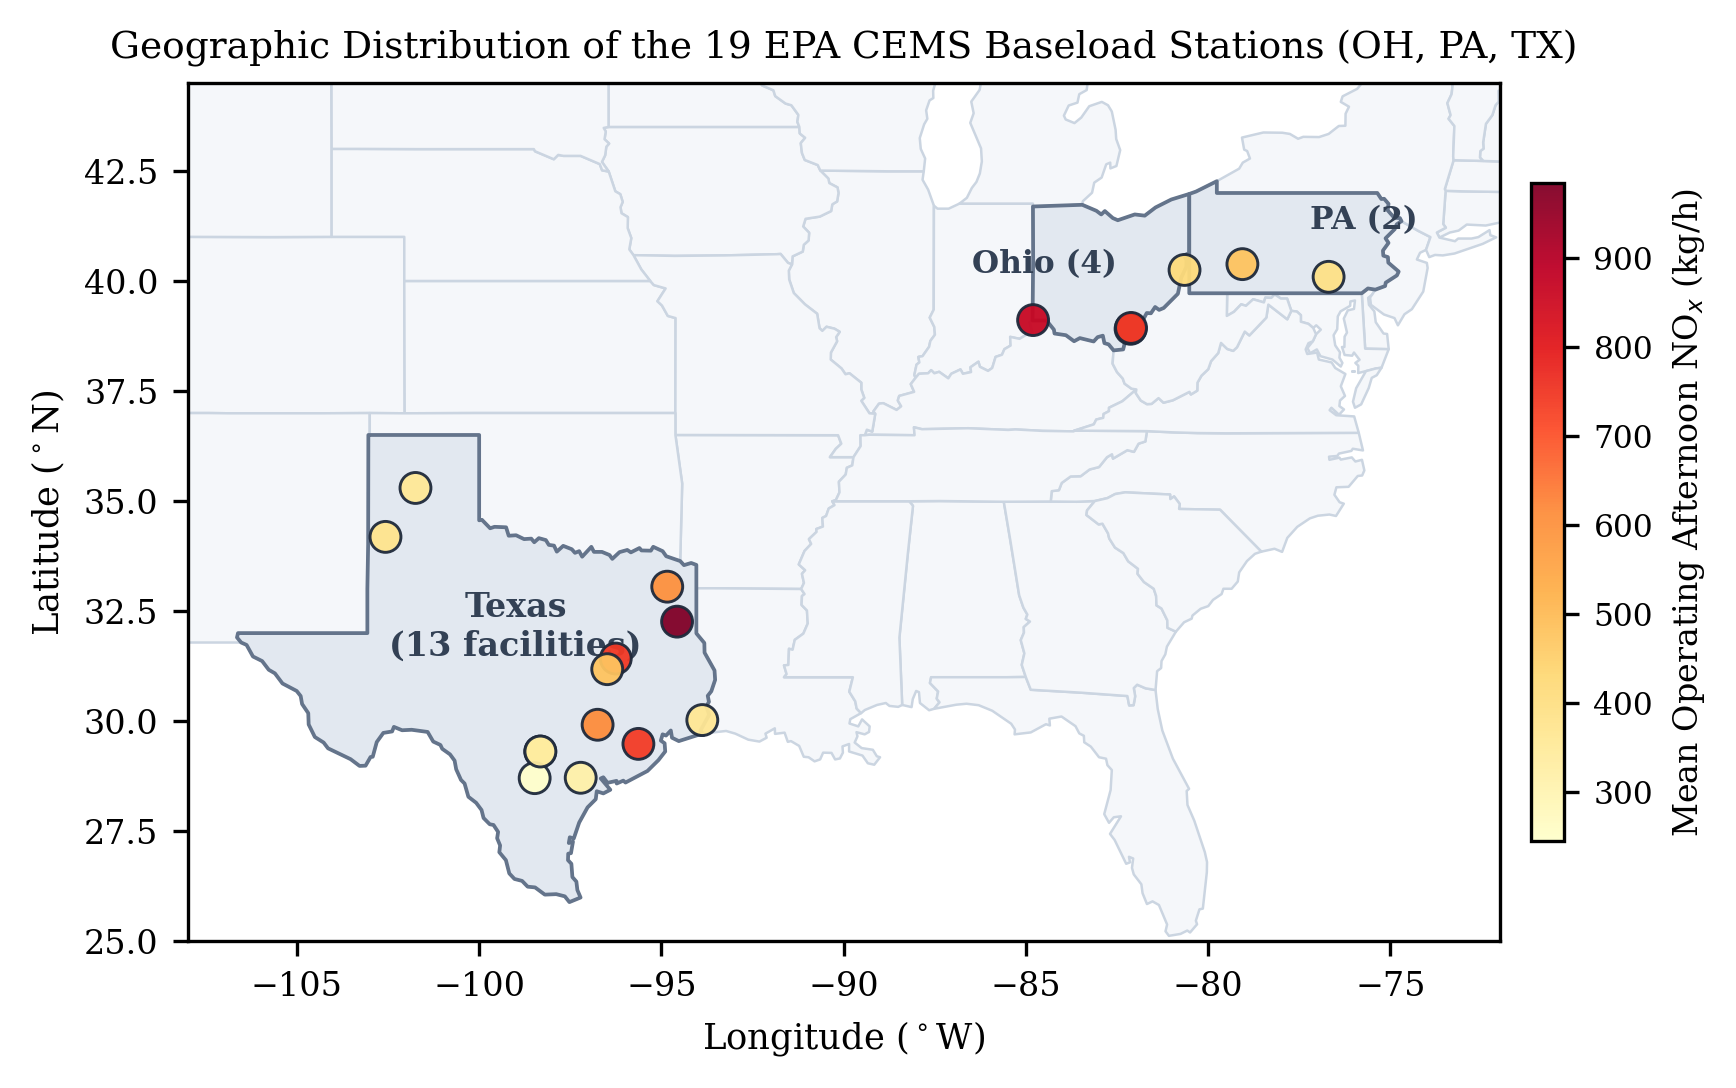
\includegraphics[width=\columnwidth]{figures/fig_facilities_map.png}
\caption{Geographic distribution of the \NFacilities~EPA CEMS facilities in Ohio, Pennsylvania, and Texas selected by the objective baseload completeness rule, colored by mean afternoon $\text{NO}_x$ emission rate ($\text{kg/h}$). Coordinates from EIA Form~860.}
\label{fig:map}
\end{figure}

\subsection{ERA5 Meteorology and Timezone Alignment}
For each facility's EIA-860 coordinates, \texttt{src/data/fetch\_era5.py} queries the Open-Meteo ERA5 reanalysis archive (\texttt{models=era5}) with explicit unit and clock parameters (\texttt{wind\_speed\_unit=ms}, \texttt{timezone=GMT}). We retrieve 10.0\,m wind speed ($\text{m/s}$), 10.0\,m wind direction (degrees meteorological, blowing \textit{from}), surface pressure ($\text{hPa}$), 2\,m temperature ($^\circ\text{C}$), and planetary boundary-layer height ($\text{m}$). ERA5 UTC timestamps are shifted by each state's standard-time offset ($\text{OH}: -5\text{ h}$, $\text{PA}: -5\text{ h}$, $\text{TX}: -6\text{ h}$) prior to an exact one-to-one join on \texttt{(Facility ID, Date, Hour)}. Across all \NFacilityHours~synchronized facility-hours (\NOperatingHours~operating with complete $\text{NO}_x$ and \NNonOperatingHours~non-operating), the verified mean 10.0\,m wind speed is \MeanWindSpeed~$\text{m/s}$, and the mean (median) operating $\text{NO}_x$ rate is \MeanNOx~kg/h (\MedianNOx~kg/h). Eastward and northward wind components are computed via $u = -w \sin\theta$ and $v = -w \cos\theta$.

\subsection{Consecutive Sequence Windows}
The module \texttt{src/data/dataset.py} maps calendar days and overpass hours ($13$ and $14\text{ LST}$) to contiguous integer slot indices. A sample is a window of $T = 4$ \textbf{strictly consecutive} slots at a single facility (i.e., 13:00 and 14:00~LST on two consecutive calendar days) whose final slot is an operating hour with complete $\text{NO}_x$. Any window spanning a calendar gap or missing meteorological record is discarded, yielding \NWindows~valid windows across the \NFacilities~facilities.

\section{Methodology}
\label{sec:method}

\subsection{Input Feature Sets}
Each window is a tensor $\mathbf{X} \in \mathbb{R}^{T \times F}$ with $T = 4$. We evaluate two feature sets:
\begin{enumerate}
    \item \textbf{Weather + Load ($F = 10$)}: $\mathbf{m}_t = [u_t, v_t, w_t, P_t, T_{2\text{m},t}, \text{PBLH}_t]$ (6 meteorological variables), seasonal/hour encodings $[\sin(2\pi\,\text{month}/12), \cos(2\pi\,\text{month}/12), \mathbb{I}(\text{Hour}=14)]$, and facility gross load $L_t$ ($\text{MW}$).
    \item \textbf{Weather Only ($F = 9$)}: Identical to above but omitting gross load $L_t$, isolating how much variance can be explained by meteorology and calendar context alone.
\end{enumerate}
All features are standardized using the per-feature mean and standard deviation computed \textbf{exclusively on the training fit split} of each fold: $\tilde{\mathbf{X}} = (\mathbf{X} - \boldsymbol{\mu}_{\text{fit}}) / (\boldsymbol{\sigma}_{\text{fit}} + 10^{-6})$. The target is log-transformed emission $z = \ln(1 + y_T)$, where $y_T$ is the facility $\text{NO}_x$ release rate ($\text{kg/h}$) at slot $T$. Predictions are mapped back to physical units via $\hat{y}_T = \max(\exp(\hat{z}) - 1, 0)$.

\subsection{Meteorological Coupling and Combustion Telemetry}
\label{sec:physics_coupling}
In baseload utility boilers, ambient meteorological variables are hypothesized to interact with operational telemetry through three physical and thermodynamic pathways (which serve as domain motivation rather than isolated causal effects verified by ablation):
\begin{enumerate}
    \item \textbf{Combustion Air Density and Humidity}: Ambient temperature and surface pressure govern combustion air mass density and oxygen stoichiometry, which we hypothesize may influence flame zone peak temperatures driving thermal $\text{NO}_x$ generation via the extended Zeldovich mechanism~\cite{beirle2019pinpointing}.
    \item \textbf{Post-Combustion SCR Catalyst Temperature}: Selective catalytic reduction (SCR) systems require flue-gas temperatures within an operational window ($315^\circ\text{C}$ to $400^\circ\text{C}$) for catalytic $\text{NO}_x$ reduction; we hypothesize that ambient winter temperatures and cold boiler startups alter ductwork heat-loss rates, although stack-level telemetry cannot directly verify internal catalyst temperatures.
    \item \textbf{Weather-Driven Dispatch Demand}: Local temperature extremes (summer cooling and winter heating) drive grid dispatch setpoints, determining boiler ramping rates and unit operating states. Downwind atmospheric plume dispersion and buoyant plume rise~\cite{defoy2015estimating,goldberg2022using} govern satellite column concentrations downwind (Phase~B), whereas Phase~A focuses on stack-level emissions.
\end{enumerate}

\subsection{AirCross Architecture}
Given a normalized window $\tilde{\mathbf{X}} \in \mathbb{R}^{T \times F}$, AirCross (\texttt{src/models/aircross.py}) projects each time slot to dimension $D = 64$ with learned positional embeddings $\mathbf{P} \in \mathbb{R}^{1 \times T \times D}$ and applies $L = 2$ pre-norm Transformer encoder layers ($H = 4$ heads, GELU activation, dropout $0.1$):
\begin{equation}
    \mathbf{H} = \text{TransformerEncoder}(\tilde{\mathbf{X}}\mathbf{W}_{\text{in}} + \mathbf{P}) \in \mathbb{R}^{T \times D}.
\end{equation}
To condition multi-hour dispatch history on the instantaneous dispersion environment, the 6 normalized meteorological variables at the target overpass slot $\tilde{\mathbf{m}}_T \in \mathbb{R}^{1 \times 6}$ are projected into query vector $\mathbf{q} = \tilde{\mathbf{m}}_T \mathbf{W}_q \in \mathbb{R}^{1 \times D}$ that attends over $\mathbf{H}$ via multi-head cross-attention:
\begin{equation}
    \mathbf{c} = \text{MHA}(\text{query}=\mathbf{q},\,\text{key}=\mathbf{H},\,\text{value}=\mathbf{H}) \in \mathbb{R}^{1 \times D}.
\end{equation}
Physically, the temporal tokens $\mathbf{H}$ encode internal plant operating inertia (multi-hour fuel feed dynamics and boiler thermal ramp), whereas the query $\mathbf{q}$ isolates the external atmospheric state (wind dispersion vectors and boundary-layer mixing height) into which stack effluents are discharged at the target overpass hour.
A residual connection with the final token $\mathbf{h}_T$ followed by LayerNorm and a two-layer MLP head yields the prediction:
\begin{equation}
    \hat{z} = \text{MLP}(\text{LN}(\mathbf{c} + \mathbf{h}_T)).
\end{equation}
In the \textbf{AirCross (no cross-attention)} ablation, $\mathbf{c}$ is omitted and $\text{LN}(\mathbf{h}_T)$ is passed directly to the MLP head.

\subsection{Baselines and Training Protocol}
All models receive the exact same windows and splits (\texttt{src/models/baselines.py}):
\begin{itemize}
    \item \textbf{Global mean}: Predicts the mean training $y$ ($\text{kg/h}$).
    \item \textbf{Per-facility mean}: Predicts each facility's training mean $y$ (defined only on the temporal split).
    \item \textbf{Load regression}: Ordinary least squares $y_T = \alpha + \beta L_T$ fitted in $\text{kg/h}$ on target gross load.
    \item \textbf{Histogram Gradient Boosting}: \texttt{HistGradientBoostingRegressor} with fixed defaults (400 trees, learning rate $0.05$, max leaf nodes $31$, seed~0) fitted on flattened windows $\mathbb{R}^{T \cdot F}$ with target $\ln(1+y_T)$.
    \item \textbf{MLP and 1D-CNN}: Neural baselines with identical loss, optimizer, early stopping, and learning-rate schedule as AirCross.
\end{itemize}
Neural models minimize Smooth-$L_1$ loss on $\ln(1+y_T)$ using AdamW ($\text{lr} = 10^{-3}$, weight decay $10^{-4}$, batch size $256$, gradient clip $1.0$), \texttt{ReduceLROnPlateau} (factor $0.5$, patience $2$), and early stopping on validation loss (patience $6$, maximum $60$ epochs), restoring the best validation checkpoint. Neural models are trained across \textbf{\NSeeds~random seeds} ($\{0, 1, 2, 3, 4\}$).

\section{Experimental Setup and Results}
\label{sec:results}

\subsection{Evaluation Splits and Cluster Isolation}
We evaluate two generalization regimes:
\begin{enumerate}
    \item \textbf{Temporal Hold-Out (Future Years)}: Across all \NFacilities~facilities, 2020--2022 forms the fit set, 2023 is the validation set for early stopping, and 2024--2025 is the held-out test set.
    \item \textbf{Spatial Hold-Out (50~km Cluster-Independent 5-Fold Grouped CV)}: To prevent geographic data leakage between co-located power stations (e.g., Kyger Creek and Gavin are 2.5~km apart in Cheshire, OH; Sommers and Spruce are 0.4~km apart in San Antonio, TX; Limestone and Oak Grove are \MaxClusterDistKm{}~km apart), facilities within 50~km are grouped into \NClusters{} connected spatial clusters. These clusters are partitioned across \NFolds~disjoint folds (\texttt{spatial\_split\_seed: 42}; fold assignments in Table~\ref{tab:facilities}), ensuring that no facility in a test fold is within 50~km of any facility in the training folds. In each fold, training facilities use 2020--2022 for fitting and 2023 for validation early stopping.
\end{enumerate}
We report MAE ($\text{kg/h}$), root mean squared error (RMSE, $\text{kg/h}$), coefficient of determination ($R^2$), scale-free log-MAE, and mean prediction bias ($\text{mean}(\hat{y} - y)$). For spatial cross-validation, to account for spatial error covariance between adjacent facilities, statistical inference is conducted via 2,000-replicate paired geographic cluster bootstrap resampling. The resampling unit is strictly the \NClusters{} disjoint geographic clusters (not individual facilities); in each bootstrap replicate, an identical set of resampled clusters is evaluated across models, computing paired difference distributions $\Delta\text{MAE} = \text{MAE}_{\text{model}} - \text{MAE}_{\text{LoadReg}}$. Under \NClusters{} geographic clusters, the two-sided minimum detectable effect size at $\alpha = 0.05$ with $80\%$ power is $\approx \pm \MinDetectableEffectKgH\text{ kg/h}$ ($\approx \MinDetectableEffectPct\%$ of baseline MAE).

\subsection{Temporal Generalization Results (2024--2025)}
Table~\ref{tab:temporal} reports performance on the 2024--2025 temporal hold-out, and Fig.~\ref{fig:pred_vs_obs} illustrates observed versus predicted $\text{NO}_x$ rates.
\begin{itemize}
    \item \textbf{Baseline Comparison}: The global training mean exhibits an MAE of \TempGlobalMeanMAE~kg/h ($R^2 = \TempGlobalMeanR$), and linear load regression reduces MAE to \TempLoadRegMAE~kg/h ($R^2 = \TempLoadRegR$). Per-facility training means reach \TempFacMeanMAE~kg/h ($R^2 = \TempFacMeanR$), reflecting persistent baseline differences across facilities.
    \item \textbf{Model Performance}: Histogram gradient boosting achieves the lowest temporal error at \textbf{\TempGBMAE~kg/h} ($R^2 = \TempGBR$). AirCross achieves \textbf{\TempAirCrossMAE~$\pm$~\TempAirCrossMAEsd~kg/h} ($\text{RMSE} = \TempAirCrossRMSE$~kg/h, $R^2 = \TempAirCrossR$, $\text{logMAE} = \TempAirCrosslogMAE$), reducing MAE by \TempAirCrossVsGlobalPct\% relative to the global mean and by \TempAirCrossVsLoadRegPct\% relative to linear load regression. 1D-CNN and MLP achieve \TempCNNMAE~$\pm$~\TempCNNMAEsd~kg/h and \TempMLPMAE~$\pm$~\TempMLPMAEsd~kg/h, respectively.
\end{itemize}

\begin{table}[htbp]
\caption{Temporal hold-out: train 2020--2022, early stopping on 2023, test 2024--2025 (all facilities). Errors in kg/h NO$_x$; mean $\pm$ s.d. over seeds where applicable. Bias = mean($\hat{y} - y$).}
\label{tab:temporal}
\centering
\footnotesize
\setlength{\tabcolsep}{2.5pt}
\resizebox{\columnwidth}{!}{
\begin{tabular}{lccccc}
\toprule
\textbf{Model} & \textbf{MAE} & \textbf{RMSE} & \textbf{$R^2$} & \textbf{logMAE} & \textbf{Bias} \\
\midrule
Global mean & 301.6 & 384.9 & -0.029 & 0.687 & 64.7 \\
Per-facility mean & 259.2 & 348.9 & 0.154 & 0.586 & 62.9 \\
Load regression & 209.1 & 282.8 & 0.445 & 0.481 & 26.9 \\
Gradient boosting & \textbf{160.1} & 238.8 & 0.604 & 0.361 & -16.2 \\
MLP & 180.1 $\pm$ 3.6 & 261.3 $\pm$ 4.4 & 0.526 $\pm$ 0.016 & 0.401 $\pm$ 0.007 & -23.3 $\pm$ 9.4 \\
1D-CNN & 175.0 $\pm$ 3.1 & 257.4 $\pm$ 5.7 & 0.540 $\pm$ 0.020 & 0.390 $\pm$ 0.005 & -33.9 $\pm$ 9.5 \\
AirCross (no cross-attention) & 179.0 $\pm$ 5.3 & 256.8 $\pm$ 8.3 & 0.541 $\pm$ 0.030 & 0.394 $\pm$ 0.010 & 0.0 $\pm$ 16.4 \\
AirCross & 170.7 $\pm$ 3.0 & 255.6 $\pm$ 6.0 & 0.546 $\pm$ 0.021 & 0.378 $\pm$ 0.005 & -32.9 $\pm$ 17.0 \\
\bottomrule
\end{tabular}
}
\end{table}


\begin{figure}[htbp]
\centering
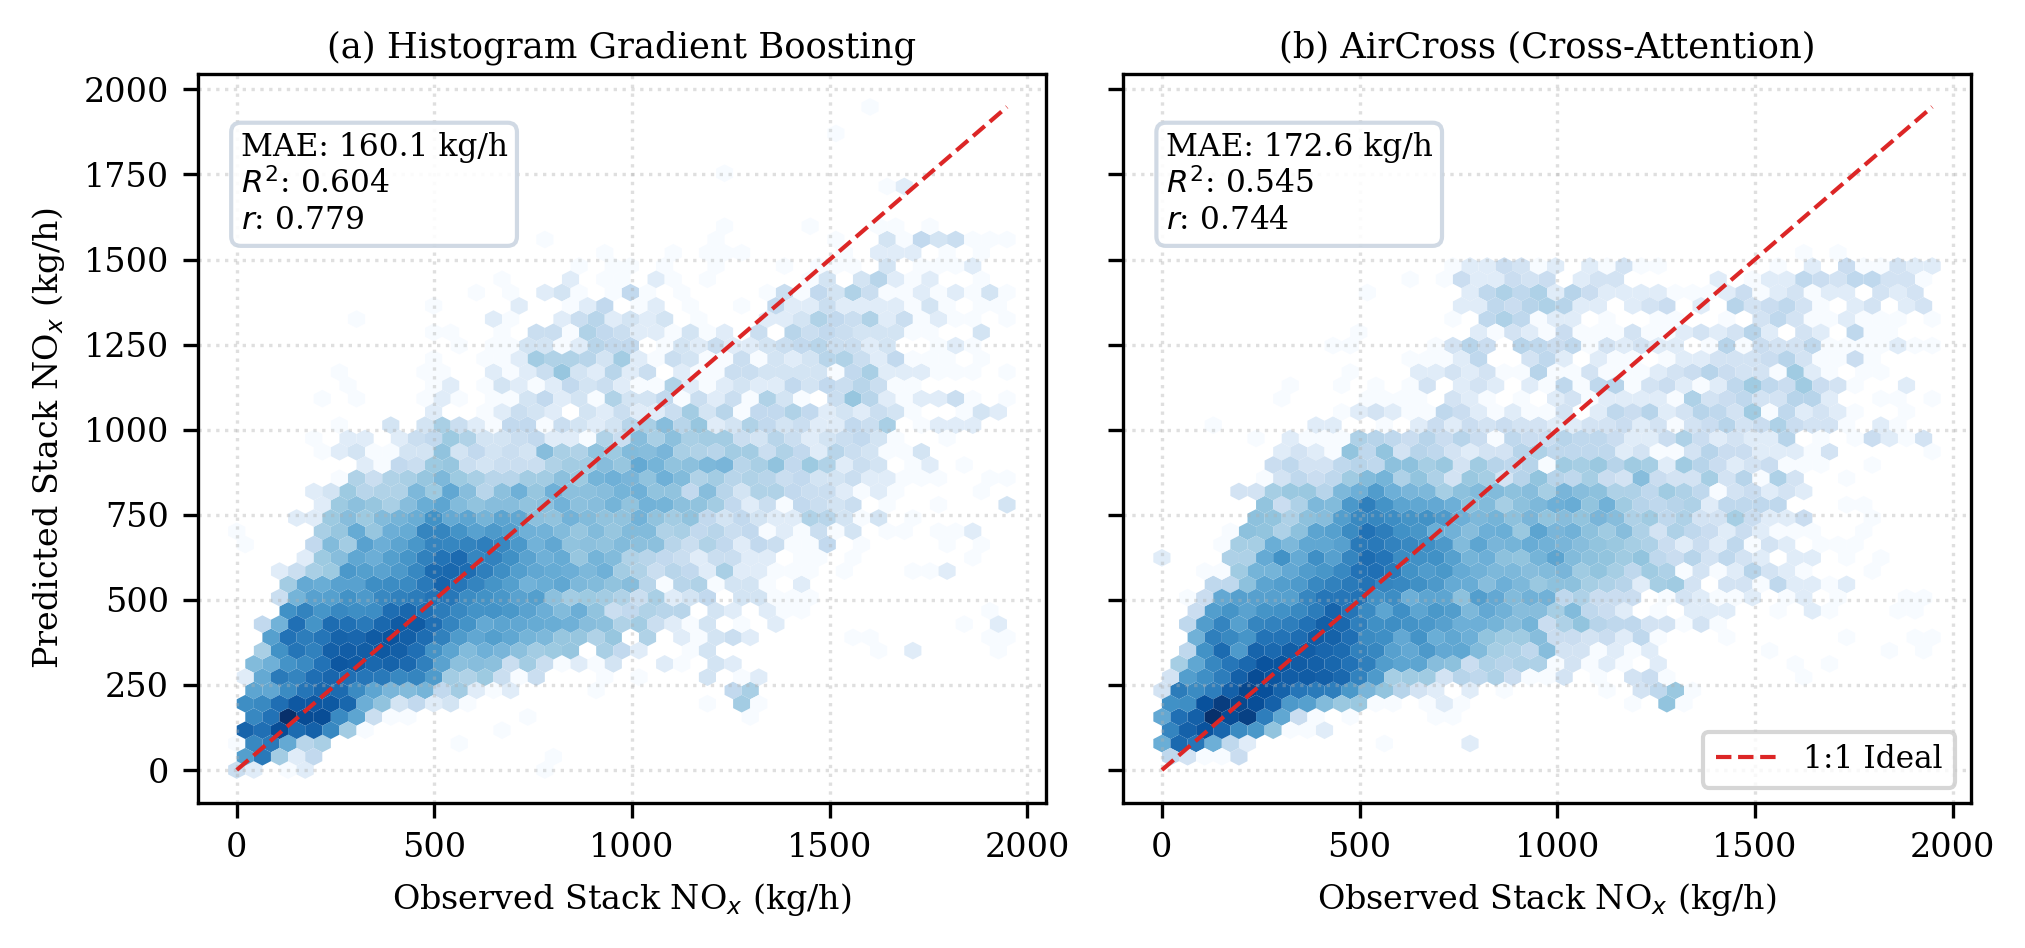
\includegraphics[width=\columnwidth]{figures/fig_pred_vs_obs.png}
\caption{Observed versus predicted afternoon $\text{NO}_x$ emission rates ($\text{kg/h}$) on the 2024--2025 temporal test split for Gradient Boosting and AirCross (seed~0).}
\label{fig:pred_vs_obs}
\end{figure}

\subsection{Spatial Generalization Results (Unseen Facility Clusters)}
Table~\ref{tab:spatial} and Fig.~\ref{fig:spatial_pf} present the cluster-independent spatial cross-validation results across unseen facility clusters.
\begin{itemize}
    \item \textbf{Comparison on Unseen Plants}: Across completely unseen facilities, MLP achieves an MAE of \textbf{\SpatMLPMAE~$\pm$~\SpatMLPMAEsd~kg/h}, followed closely by gradient boosting (\textbf{\SpatGBMAE~kg/h}) and linear load regression (\textbf{\SpatLoadRegMAE~kg/h}), with 1D-CNN at \SpatCNNMAE~$\pm$~\SpatCNNMAEsd~kg/h and AirCross at \SpatAirCrossMAE~$\pm$~\SpatAirCrossMAEsd~kg/h.
    \item \textbf{Absence of Detectable Difference Under Geographic Cluster Bootstrap}: Paired geographic cluster bootstrap difference tests against linear load regression reveal that the 95\% confidence intervals for all learned models span zero: MLP vs.\ LoadReg has $\Delta\text{MAE} \in [\SpatMLPdCIlo, \SpatMLPdCIhi]$~kg/h, Gradient Boosting vs.\ LoadReg has $\Delta\text{MAE} \in [\SpatGBdCIlo, \SpatGBdCIhi]$~kg/h, and AirCross vs.\ LoadReg has $\Delta\text{MAE} \in [\SpatAirCrossdCIlo, \SpatAirCrossdCIhi]$~kg/h. While intervals spanning zero do not prove formal mathematical equivalence (which would require pre-specified equivalence testing margins), they establish that no statistically detectable performance advantage exists among load-aware models given the \NClusters{} geographic clusters (minimum detectable effect size $\approx \pm \MinDetectableEffectKgH\text{ kg/h}$ or $\approx \MinDetectableEffectPct\%$ of MAE). Crucially, load-conditioned models significantly outperform the unconditioned global mean (\SpatGlobalMeanMAE~kg/h, $\Delta\text{MAE} \in [\SpatGlobalMeandCIlo, \SpatGlobalMeandCIhi]$~kg/h).
    \item \textbf{Prediction Bias Analysis}: Neural models trained on $\ln(1+y)$ with Smooth-$L_1$ loss exhibit mild negative bias (\SpatCNNBias~to~\SpatMLPBias~kg/h) because $\text{expm1}$ of $L_1$-minimized predictions estimates the conditional geometric median, under-predicting extreme positive emission spikes. In contrast, linear load regression fits the arithmetic mean directly, yielding a positive bias of +\SpatLoadRegBias~kg/h.
\end{itemize}

\begin{table*}[htbp]
\caption{Spatial hold-out: grouped 5-fold cross-validation over 50~km spatial clusters (every cluster is unseen in exactly one fold; all years). 95\% CI by geographic cluster bootstrap. $\Delta$MAE: paired bootstrap difference vs.\ Load Regression. MAE$_{24\text{--}25}$: unseen facilities in 2024--2025 only.}
\label{tab:spatial}
\centering
\footnotesize
\setlength{\tabcolsep}{2.5pt}
\resizebox{\textwidth}{!}{
\begin{tabular}{lccccccc}
\toprule
\textbf{Model} & \textbf{MAE} & \textbf{RMSE} & \textbf{$R^2$} & \textbf{Bias} & \textbf{MAE 95\% CI} & \textbf{$\Delta$MAE vs LoadReg} & \textbf{MAE$_{24\text{--}25}$} \\
\midrule
Global mean & 304.6 & 390.3 & -0.048 & 33.6 & [258.4, 360.4] & [+33.5, +138.8] & 308.1 \\
Load regression & 216.4 & 293.3 & 0.408 & 22.7 & [166.2, 272.2] & 0.0 (ref) & 218.2 \\
Gradient boosting & 207.0 & 294.9 & 0.402 & -17.5 & [161.2, 258.6] & [-26.2, +8.9] & 204.5 \\
MLP & \textbf{205.6 $\pm$ 2.5} & 307.5 $\pm$ 7.0 & 0.349 $\pm$ 0.029 & -38.2 $\pm$ 5.0 & [155.4, 264.5] & [-32.0, +14.1] & 199.6 $\pm$ 2.8 \\
1D-CNN & 210.2 $\pm$ 3.0 & 304.1 $\pm$ 3.3 & 0.364 $\pm$ 0.014 & -33.0 $\pm$ 8.1 & [163.0, 265.4] & [-23.3, +11.9] & 201.6 $\pm$ 3.7 \\
AirCross (no cross-attention) & 214.6 $\pm$ 3.0 & 308.0 $\pm$ 4.4 & 0.347 $\pm$ 0.019 & -14.1 $\pm$ 9.2 & [166.6, 271.0] & [-17.3, +14.2] & 209.1 $\pm$ 4.1 \\
AirCross & 217.5 $\pm$ 5.8 & 314.8 $\pm$ 5.5 & 0.318 $\pm$ 0.024 & -36.6 $\pm$ 14.1 & [167.8, 275.2] & [-17.8, +22.5] & 212.2 $\pm$ 6.0 \\
\bottomrule
\end{tabular}
}
\end{table*}


\begin{figure}[htbp]
\centering
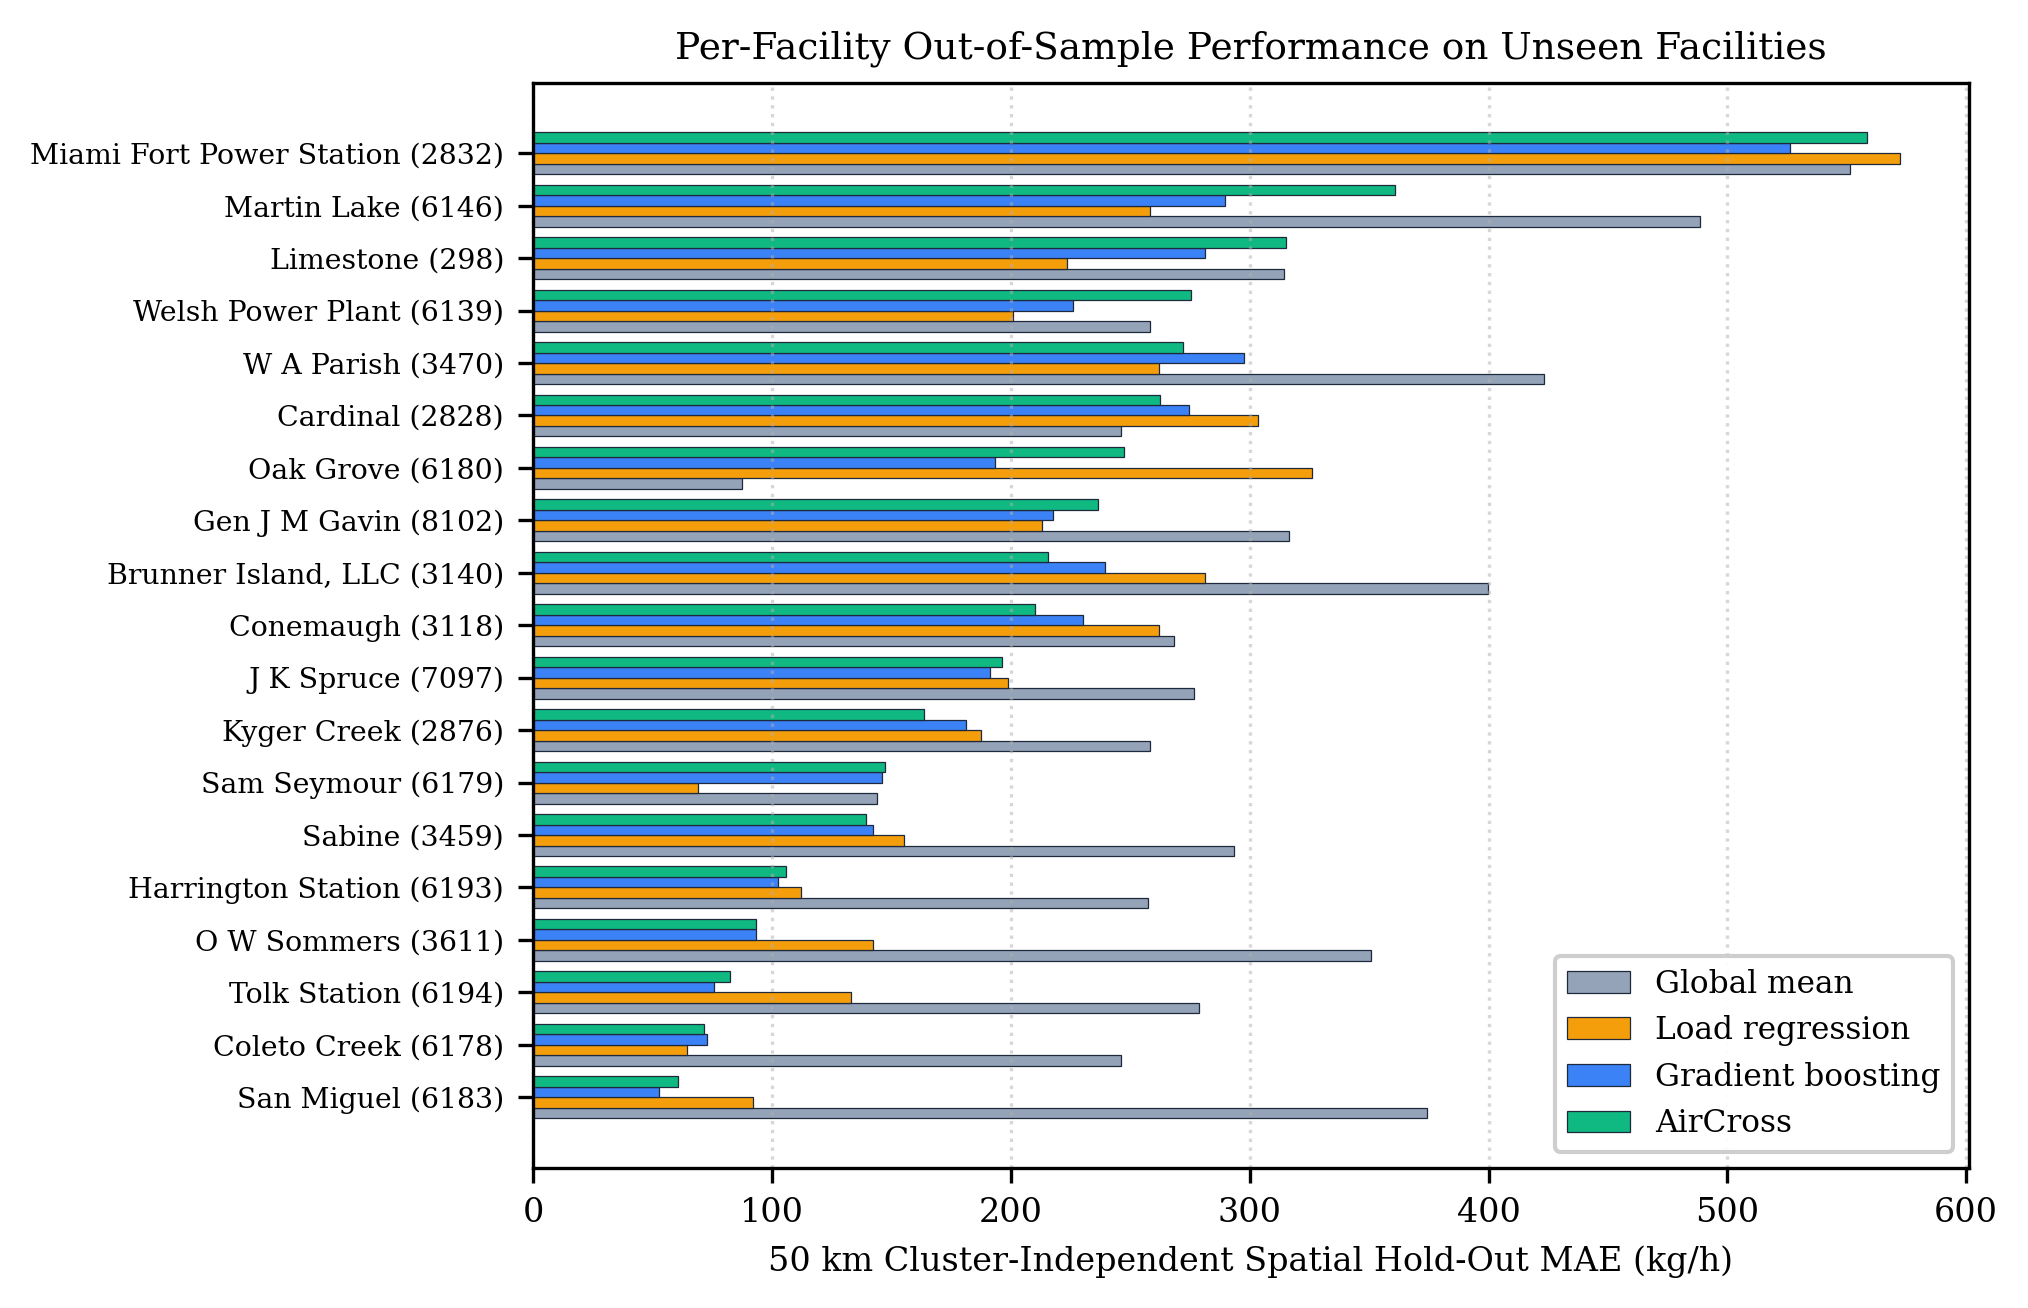
\includegraphics[width=\columnwidth]{figures/fig_spatial_per_facility.png}
\caption{Per-facility out-of-sample MAE ($\text{kg/h}$) under cluster-independent spatial cross-validation for the Global Mean, Load Regression, Gradient Boosting, and AirCross.}
\label{fig:spatial_pf}
\end{figure}

\subsection{Atmospheric Wind and Regional Subgroup Analysis}
\label{sec:subgroups}
To investigate model sensitivity under contrasting operational and atmospheric conditions, we evaluate the temporal holdout across two descriptive subgroupings (with evaluation based on the 5-seed averaged predictions):
\begin{enumerate}
    \item \textbf{Wind-Speed Regimes (Advective vs.\ Stagnant)}: In calm conditions ($w < 2.0\text{ m/s}$, $N = \NCalmTestWindows$~test sequences), absolute prediction errors are higher across all architectures (Per-Facility Mean: \RegimeFacMeanCalmMAE~kg/h; Load Regression: \RegimeLoadRegCalmMAE~kg/h; AirCross: \RegimeAirCrossCalmMAE~kg/h; Gradient Boosting: \RegimeGBCalmMAE~kg/h). Under advective conditions ($w \ge 2.0\text{ m/s}$, $N = \NAdvTestWindows$~test sequences), errors are lower across the board (Per-Facility Mean: \RegimeFacMeanAdvMAE~kg/h; Load Regression: \RegimeLoadRegAdvMAE~kg/h; AirCross: \RegimeAirCrossAdvMAE~kg/h; Gradient Boosting: \RegimeGBAdvMAE~kg/h). Gradient boosting maintains the lowest MAE across both wind regimes, while linear load regression improves by \RegimeLoadRegAdvGainMAE~kg/h and AirCross improves by \RegimeAirCrossAdvGainMAE~kg/h, showing that lower errors under advective winds reflect overall sample conditions rather than an architecture-specific transport advantage (Fig.~\ref{fig:regime_breakdown}(a)).
    \item \textbf{Regional Fleets (Texas ERCOT vs.\ PJM / Ohio-PA Fleet)}: As depicted in Fig.~\ref{fig:regime_breakdown}(b), performance differs noticeably across the two geographic fleets. In the Texas fleet ($N = \NTxTestWindows$ across \NTxPlants{} plants), where baseload units operate with lower baseline emission intensity, the per-facility mean baseline incurs \RegimeFacMeanTxMAE~kg/h, load regression achieves \RegimeLoadRegTxMAE~kg/h, AirCross achieves \RegimeAirCrossTxMAE~kg/h, and gradient boosting achieves \RegimeGBTxMAE~kg/h (paired bootstrap difference AirCross vs.\ Gradient Boosting: [\RegimeTXDiffAirCrossGBlo, \RegimeTXDiffAirCrossGBhi]~kg/h). In the PJM / Ohio-PA fleet ($N = \NMidwestTestWindows$ across \NMidwestPlants{} baseload plants), where mean emission rates are higher and unit-level capacities vary substantially, the per-facility mean incurs \RegimeFacMeanMidwestMAE~kg/h and pooled linear load regression incurs \RegimeLoadRegMidwestMAE~kg/h MAE. Here, gradient boosting (\RegimeGBMidwestMAE~kg/h) and AirCross (\RegimeAirCrossMidwestMAE~kg/h) are closely matched and statistically tied (difference 95\% CI: [\RegimeMWDiffAirCrossGBlo, \RegimeMWDiffAirCrossGBhi]~kg/h), reducing MAE by \RegimeGBMidwestGainMAE~kg/h (\RegimeGBMidwestVsLoadRegPct\%) and \RegimeAirCrossMidwestGainMAE~kg/h (\RegimeAirCrossMidwestVsLoadRegPct\%) respectively relative to pooled linear regression. This separation is primarily attributable to facility-level technological heterogeneity across the regional plants that a single pooled linear slope cannot accommodate, rather than confirmed atmospheric mechanisms.
\end{enumerate}

\begin{figure}[htbp]
\centering
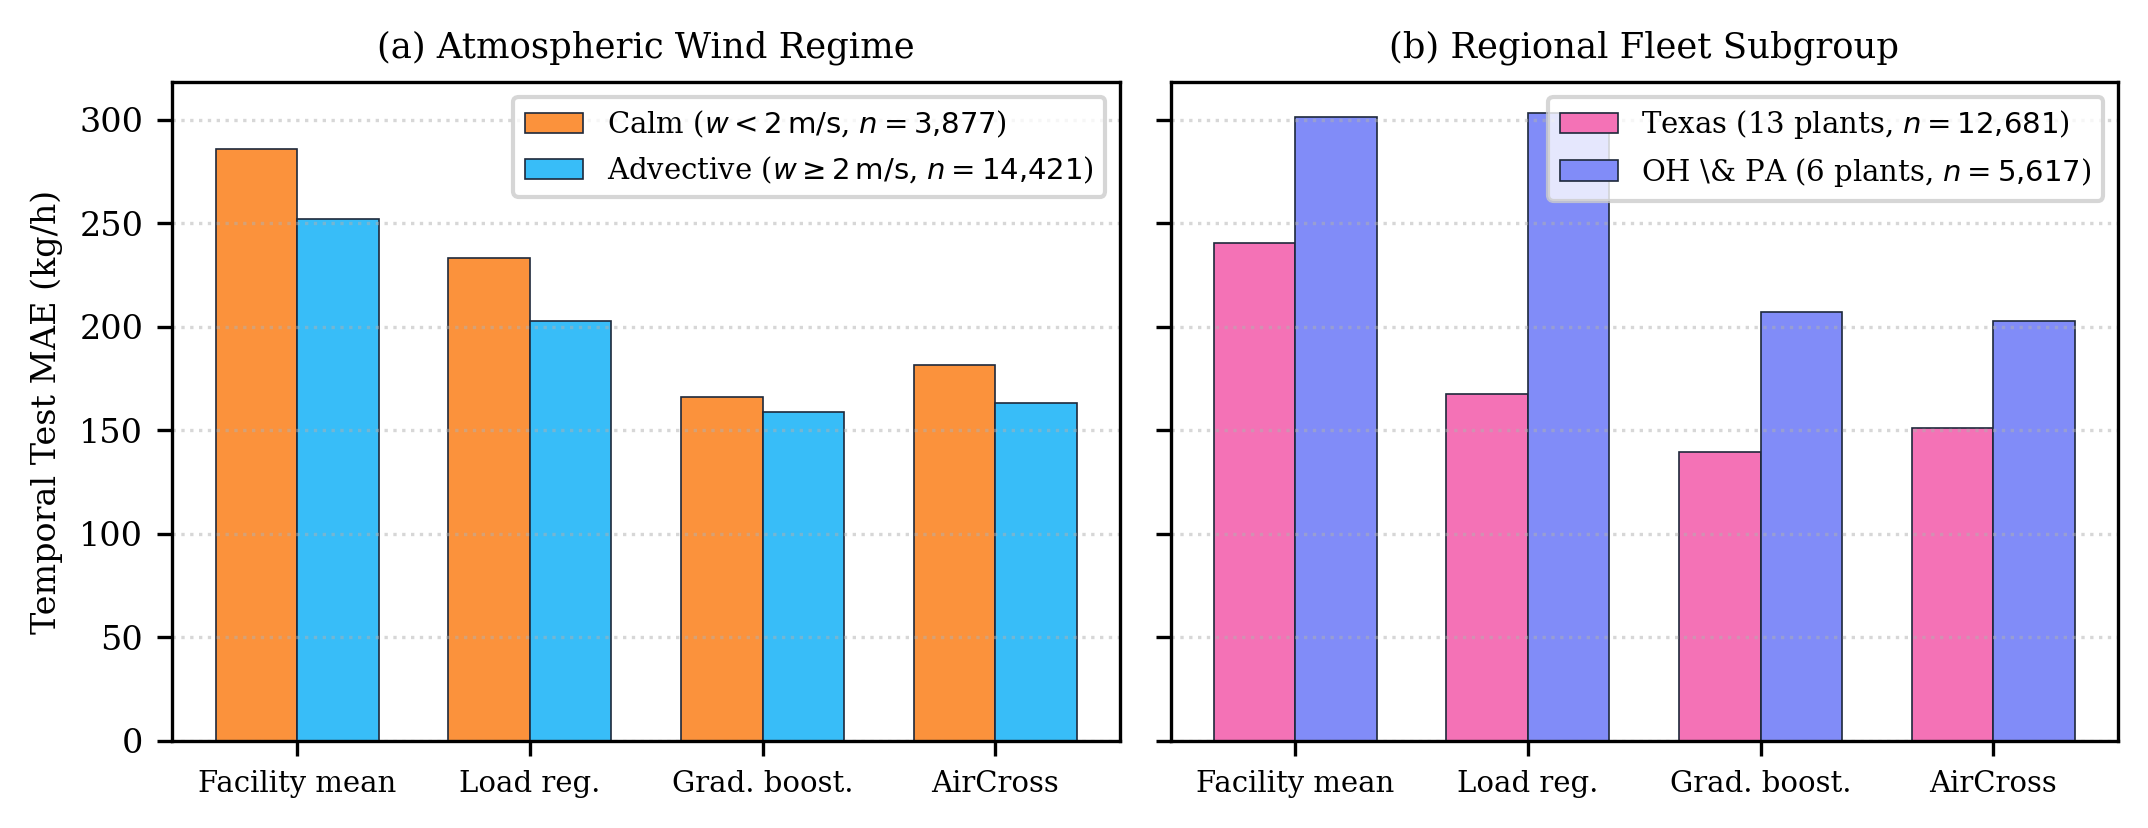
\includegraphics[width=\columnwidth]{figures/fig_regime_breakdown.png}
\caption{Temporal hold-out evaluation stratified across (a) atmospheric wind transport regimes (calm vs.\ advective) and (b) regional fleets (Texas ERCOT vs.\ Ohio/Pennsylvania PJM). AirCross values represent the 5-seed ensemble mean; Gradient Boosting is a single deterministic model.}
\label{fig:regime_breakdown}
\end{figure}

\subsection{Ablation Study: Operational Load vs.\ Meteorology}
Table~\ref{tab:ablation} isolates the predictive contribution of plant gross load and cross-attention pooling.
\begin{enumerate}
    \item \textbf{Weather-Only Generalization}: Without gross load, AirCross achieves \TempAirCrossWMAE~$\pm$~\TempAirCrossWMAEsd~kg/h temporal MAE, a \textbf{\TempWeatherOnlyVsGlobalPct\%} reduction over the global mean (\TempGlobalMeanMAE~kg/h). However, under spatial cluster hold-out, AirCross with weather only achieves \SpatAirCrossWMAE~$\pm$~\SpatAirCrossWMAEsd~kg/h, which is only a \textbf{\SpatWeatherOnlyVsGlobalPct\%} reduction over the global mean (\SpatGlobalMeanMAE~kg/h). The substantial contrast between temporal and spatial generalization suggests that weather-only models exploit persistent geographic and microclimatic signatures (such as characteristic surface pressure and elevation gradients) associated with monitored facilities across time. Under strict spatial hold-out, these site-specific topoclimatic proxies fail to transfer to unobserved boiler configurations, demonstrating the limited spatial generalizability of meteorology alone in the absence of operational gross load.
    \item \textbf{Contribution of Gross Load}: Supplying gross load reduces AirCross MAE by \textbf{\TempLoadGainPct\%} temporally and \textbf{\SpatLoadGainPct\%} spatially, confirming that electrical generation is the primary physical determinant of stack mass emissions.
    \item \textbf{Cross-Attention Pooling}: On the temporal split, cross-attention provides a modest refinement over the attention-free ablation (\TempAirCrossMAE{} vs.\ \TempAirCrossNoXMAE{}~kg/h). On unseen spatial clusters, both variants perform within seed standard deviation (\SpatAirCrossMAE{} $\pm$ \SpatAirCrossMAEsd{} vs.\ \SpatAirCrossNoXMAE{} $\pm$ \SpatAirCrossNoXMAEsd{}~kg/h).
\end{enumerate}

\begin{table}[htbp]
\caption{Ablations: input features and cross-attention pooling (MAE, kg/h, mean $\pm$ s.d. over seeds).}
\label{tab:ablation}
\centering
\footnotesize
\resizebox{\columnwidth}{!}{
\begin{tabular}{llcc}
\toprule
\textbf{Model} & \textbf{Inputs} & \textbf{Temporal} & \textbf{Spatial} \\
\midrule
Gradient boosting & weather & 250.6 & 301.6 \\
Gradient boosting & weather + load & 160.1 & 207.0 \\
AirCross & weather & 249.0 $\pm$ 3.0 & 299.7 $\pm$ 3.6 \\
AirCross (no cross-attention) & weather + load & 179.0 $\pm$ 5.3 & 214.6 $\pm$ 3.0 \\
AirCross & weather + load & 170.7 $\pm$ 3.0 & 217.5 $\pm$ 5.8 \\
\bottomrule
\end{tabular}
}
\end{table}


\section{Limitations and Phase~B Roadmap}
\label{sec:limitations}
We emphasize four limitations of Phase~A:
\begin{enumerate}
    \item \textbf{Absence of Satellite Column Retrievals}: Phase~A models operate strictly on in-situ CEMS telemetry and ERA5 reanalysis; they do not ingest Sentinel-5P TROPOMI scenes and cannot perform plume source localization or satellite-only attribution. Prototype spatial Vision Transformer and cross-sectional flux modules are isolated in \texttt{src/models/phase\_b/} for Phase~B.
    \item \textbf{Unobserved Technological Covariates}: While EIA-860 provides coordinates and gross load, differences in fuel grade (coal vs.\ gas) and post-combustion controls (selective catalytic reduction vs.\ low-$\text{NO}_x$ burners) are not explicitly conditioned as input features, contributing to the wide facility bootstrap confidence intervals (Table~\ref{tab:spatial}).
    \item \textbf{Continuous Sampling Without Cloud Masking}: Observations are sampled daily at 13:00--14:00~LST regardless of cloud cover, whereas satellite overpasses require clear-sky conditions (TROPOMI cloud fraction $< 0.3$, QA $> 0.75$).
    \item \textbf{Reanalysis Spatial Scale}: ERA5 variables represent a $0.25^\circ$ surface grid ($\approx 25\text{ km}$) and 10.0\,m anemometer level rather than effective stack plume injection height.
\end{enumerate}

\section{Data Availability}
\label{sec:data_availability}
All data supporting the findings of this study are publicly available from authoritative public repositories. Continuous Emission Monitoring System (CEMS) hourly stack telemetry is accessible via the US Environmental Protection Agency (EPA) Clean Air Markets Program Data (CAMPD) portal (\url{https://campd.epa.gov/}). Power plant technical attributes, prime mover classifications, and plant geographic coordinates are published under US Energy Information Administration (EIA) Form EIA-860 Schedule~2 (\url{https://www.eia.gov/electricity/data/eia860/}). Hourly surface and atmospheric boundary-layer meteorology are derived from the European Centre for Medium-Range Weather Forecasts (ECMWF) ERA5 reanalysis and accessed via the Open-Meteo Historical Weather API (\url{https://open-meteo.com/}). All synchronization scripts, split configurations, and evaluation pipelines are maintained in the project repository (\url{https://github.com/CaceresCristhian/Aircross}).

\section{Conclusion}
\label{sec:conclusion}
We presented an empirical benchmark of operational load and meteorological conditioning for hourly power-plant $\text{NO}_x$ emissions across \NFacilities~baseload power stations (\YearFirst--\YearLast, \NFacilityHours~synchronized facility-hours, Run~\RunID). Our findings show that: (i) gross electrical load is the primary driver of stack $\text{NO}_x$, reducing MAE by \TempLoadGainPct\%--\SpatLoadGainPct\% over weather-only models; (ii) on temporal hold-out, histogram gradient boosting achieves the lowest MAE (\TempGBMAE~kg/h), with AirCross achieving \TempAirCrossMAE~$\pm$~\TempAirCrossMAEsd~kg/h; (iii) under 50~km cluster-independent spatial cross-validation, linear load regression (\SpatLoadRegMAE~kg/h), MLP (\SpatMLPMAE~kg/h), and gradient boosting (\SpatGBMAE~kg/h) perform within paired bootstrap confidence bounds of one another; (iv) wind-speed subgrouping shows that all models, including simple load regression, achieve lower error under advective winds ($w \ge 2.0\text{ m/s}$); (v) regional subgroup analysis reveals that learned models yield their largest gains over pooled linear regression in the PJM / Ohio-PA fleet (\RegimeAirCrossMidwestVsLoadRegPct\% reduction), reflecting unmodelled boiler heterogeneity across facilities rather than confirmed microclimatic mechanisms; and (vi) weather-only models achieve substantial temporal gains (\TempWeatherOnlyVsGlobalPct\%), hypothesized to exploit geographic climate fingerprints, but fail to extrapolate to unseen plants (\SpatWeatherOnlyVsGlobalPct\% gain). This benchmark establishes an empirical foundation for Phase~B integration with real Sentinel-5P TROPOMI column retrievals.

\bibliographystyle{IEEEtran}
\bibliography{references}

\end{document}
